\documentclass[12pt]{article} 
\usepackage{verbatim}
\usepackage{natbib}
\usepackage{amsmath}
\usepackage{amssymb}
\usepackage{calc}
\usepackage{amsmath}
\usepackage{amssymb}
\usepackage{amsthm}
\usepackage{relsize}
\usepackage{bm}
\usepackage{hyperref}
\usepackage{tikz-cd}
\usepackage[utf8]{inputenc}
\usepackage[english]{babel}
\usepackage[margin=1in]{geometry}
\usepackage{graphicx}
\usepackage{subfigure}
%\input{Young.sty}

\newtheorem{theorem}{Theorem}[section]
\newtheorem{claim}[theorem]{Claim}
\newtheorem{proposition}[theorem]{Proposition}
\newtheorem{lemma}[theorem]{Lemma}
\newtheorem{corollary}[theorem]{Corollary}
\newtheorem{conjecture}[theorem]{Conjecture}

\newtheorem*{observation}{Observation}
\theoremstyle{definition}
\newtheorem{definition}[theorem]{Definition}
\newtheorem*{example}{Example}
\newtheorem*{remark}{Remark}
\newtheorem*{note}{Note}
\newtheorem*{exercise}{Exercise}

\title{Algebraic Topology Notes}
\author{Amal Mattoo, Carson Teitler}

\begin{document}
	\maketitle 
	\section{Monday, September 13}
	Logistics 
	\begin{itemize}
		\item Textbooks: Peter May's ``Concise Course in Algebraic Topology'' and Tom Diecks ``Algebraic Topology''
		\item Take home midterm and final
		\item Grading: for graduate students, presumably ``you get an A for being alive'' 
	\end{itemize}
	This is a modern class with high tech stuff (he doesn't like Hatcher). 
	
	Slogan: algebraic topology is the study of functors from some suitable category\footnote{Cartesian closed symmetric monoidal} of spaces to Abelian groups that 1 take homotopy equivalences to isomorphisms and 2 can often be computed inductively. 
	
	We want to solve problems in geometry by turning them into problems into algebra. Broadly, geometry is hard and geometry is easy (true to varying degrees).
	
	\begin{definition}
		A category $C$ is a collection of objects $\text{Ob}(C)$, and for each pair $X,Y\in\text{Ob}(C)$ a set\footnote{We will mostly ignore set theory complications. However, they become more relevant when it comes to localization.} $\text{Hom}(X,Y)$, along with an associative map $\text{Hom}(Y,Z)\times \text{Hom}(X,Y)\to\text{Hom}(X,Z)$, and for every $X\in\text{Ob}(C)$ there is an identity map $\text{id}_X\in\text{Hom}(X,Y)$ such that $\text{id}_{X}\circ\gamma=\gamma\circ\text{id}_{X}=\gamma$ for all maps $\gamma$. 
	\end{definition} 
	\begin{example}
		\begin{itemize}
			\item \emph{Top}: spaces with continuous maps maps
			\item \emph{Fin}: finite sets with maps of sets
			\item \emph{Ab}: abelian groups with group homomorphisms
			\item \emph{R}: rings with ring maps (likewise, R-modules with R-linear maps)
			\item (More abstract) $(\mathbf{Z},\leq)$: objects are $\mathbf{Z}$ and a map $x\to y$ whenever $x\leq y$
			\item A \emph{monoid} can be thought of as a category with a single object and some morphisms
			\item A \emph{diagram} represents objects with vertices and morphisms with arrows (usually arrows representing the identity are omitted)
		\end{itemize}
	\end{example}
	Idea: we can encode everything about an object by its relationship with other objects. 
	\begin{definition}
		In a category $C$, a map $f:X\to Y$ is an isomorphism if there exists $g:Y\to X$ with $g\circ f=\text{id}_{X}$ and $f\circ g=\text{id}_{Y}$.
	\end{definition}
	\begin{example}
		Isomorphisms in Top are homeomorphisms, in Fin they are bijections, in Ab they are isomorphisms of groups, etc.
	\end{example}
	\begin{definition}
		For categories $C,D$, a \emph{functor} is a map $F:\text{ob}(C)\to \text{ob}(D)$ and a map $\text{Hom}_{C}(X,Y)\to\text{Hom}_{C}(F(X),F(Y))$ that is compatible with composition. 
	\end{definition}
	\begin{example}
		\begin{itemize}
			\item Forgetful functors $\text{Top}\to\text{Set}$, $\text{Ab}\to\text{Set}$, $\text{Ab}\to\text{Gp}$, etc. 
			\item Functors from a diagram to other categories (i.e., specifying an object for each vertex and a morphism for each arrow)
		\end{itemize}
	\end{example}
	Returning to our slogan, we want to study functors from Top to Ab that 1 solve problems and 2 can be computed. 
	
	\begin{definition}
		A functor $F$ is \emph{full} if the map $\text{Hom}_{C}(X,Y)\to\text{Hom}_{D}(F(X),F(Y))$ is surjective, and it is \emph{faithful} if that map is injective. 
	\end{definition}
	Thus, a fully faithful functor embeds $C$ as a subcategory of $D$. 
	\begin{definition}
		A functor $F:C\to D$ is an \emph{equivalence} if $F$ is fully faithful and $F$ is essentially surjective (i.e., $\forall d\in\text{ob}(D),\exists c\in\text{ob}(C)\text{ s.t. }F(c)\cong d$).
	\end{definition}
	An equivalence of categories admits an inverse, but this might require the axiom of choice to construct.  
	
	For any category $C$, for any object $c\in C$ we have functor $\text{Hom}_{C}(c,-)$ from $C\to\text{Set}$ that takes $c'\mapsto \text{Hom}_{C}(c,c')$ and takes $f:c'\to c''$ to $\varphi\mapsto \varphi\circ f$. We can think of this as a functor $C\to\text{Fun}(C,\text{Set})$. 
		
	Likewise, there is a contravariant functor $\text{Hom}(-,c)$, which we can think of as a functor $C\to\text{Fun}(C^{\text{op}},\text{Set})$.
	
	\begin{definition}
		The functor category $\text{Fun}(C,D)$ has objects functors $C\to D$ and morphisms natural transformations $F\to G$. 
	\end{definition} 
	\begin{definition}
		A natural transformation between functors $F:C\to D$ and $G:C\to D$ is for each object $c$ a map $F(c)\to G(c)$ such that for every  $c\to c'$ the following diagram commutes.
		$$\begin{tikzcd}
				F(c) \arrow[r] \arrow[d] & G(c) \arrow[d] \\
				F(c') \arrow[r]          & G(c')         
			\end{tikzcd}$$
	\end{definition}
	\begin{lemma}[Yoneda]
		For any category $C$, the functor $F\to\text{Fun}(C^{\text{op}},\text{Set})$ taking $c\mapsto\text{Hom}_{C}(-,c)$ is fully faithful. 
	\end{lemma}
	The point is that to understand an object, it suffices to consider all the maps into it. But that's too much! This begs the question, is there a good sub-class of test spaces? Maybe... spheres? 
	
	The most basic question about a category is classification: what are the isomorphisms of $\text{ob}(C)$? E.g., for real finite-dimensional vector spaces, the answer is $\{\mathbf{R}^{n}\}_{n}$. Then, we might ask: what is the structure of the isomorphism? For real finite-dimensional vector spaces, it is $\text{GL}_{n}(\mathbf{R})$.
	
	However, for topology both these questions are far too intractable. So we need a weaker notion of equivalence. 
	\begin{definition}
		For $f,g:X\to Y$ in Top, $f,g$ are homotopic if there exists a map $H:X\times I\to Y$ such that  $H(x,0)=f(x)$ and $H(x,1)=g(x)$.
	\end{definition}
	That is, a one parameter family of maps $\gamma_{x}$ parameterized by $x\in\{0,1\}$. We may think of it un-rigorously as a continuous map $\tilde{H}:I\to\text{Hom}_{C}(X,Y)$ with $\tilde{H}(0)=f$ and $\tilde{H}(1)=g$, but the codomain is a set not a space. 
	
	If we think of Top not just as a category but as an enriched category, then $\text{Map}_T(X,Y)$ is a space and composition is continuous. We endow $\text{Map}_T(X,Y)$ with the compact-open topology: a subbase consists of, for all compact $K\subseteq X$ and open $U\subseteq y$, the set $\{f:f(K)\subseteq U\}$.
	
	In fact, the relationship between $I\xrightarrow{\tilde{H}}\text{Map}_T(X,Y)$ and $H\in\text{Map}_T(X\times I,Y)$ is the concept of an adjunction.
	\begin{definition}
		$f:X\to Y$ is a homotopy equivalence if $\exists g: Y\to X$ s.t. $f\circ g\simeq \text{id}_{Y}$ and $g\circ f\simeq \text{id}_{X}$.
	\end{definition}
	Consequences 
	\begin{enumerate}
		\item $\{S^n\}$ as test spaces are basically enough to detect homotopy equivalence 
		\item There exist nice combinatorial models of spaces up to homotopy 
	\end{enumerate}
	
	\section{Wednesday, September 15}
	Haynes Miller has good notes on algebraic topology
	
	References for Category Theory 
	\begin{itemize}
		\item ``Categories in Context'' by Emily Riehl
		\item ``Categories for the Working Mathematician'' (classic)
	\end{itemize} 
	We discussed the isomorphism of sets 
	$$\theta: \text{Map}_{T}(X\times Y,Z)\cong\text{Map}_{T}(X,\text{Map}_{T}(Y,Z)) $$
	taking $f$ to $x\mapsto f(x,-)$. We claim that $\theta$ is natural: that is, compatible with maps $X'\to X$ etc. 
	\begin{definition}
		Functors $F:C\to D$ and $G:D\to C$, are an \emph{adjunction} if there is a natural isomorphism $\text{Map}_{D}(F(x),y)\cong\text{Map}_{C}(x,G(y))$. Here, $F$ is the left adjoint and $G$ is the right adjoint. 
	\end{definition}
	Since we have a natural isomorphism $\text{Map}(Fx,Fx)\cong \text{Map}(x,GFx)$, there is a natural transformation $\text{Id}\to GF$ called the \emph{unit}. Similarly, there is a natural transformation $FG\to\text{Id}$ called the \emph{counit}. 
	\begin{example}
		Let $U:\text{groups}\to\text{sets}$ be the forgetful functor. Then $U$ is the right adjoint of a functor $F:\text{sets}\to\text{groups}$ which is the free group functor: 
		$$\text{Map}_{\text{sets}}(S,UG)\cong\text{Map}_{\text{groups}}(FS,G) $$ 
	\end{example}
	\begin{definition}
		A \emph{monad} is an endofunctor $M:C\to C$ with natural transformations $MM\to M$ and $\text{id}\to M$.
	\end{definition}
	There is an Endofunctor of sets $UF$ with the unit $\text{id}\to UF$. Then $$(UF)(UF)\cong U(FU)F\xrightarrow{counit}UF$$
	Thus, we have a monad. Let $S$ is an algebra over this monad if $\mu:UFS\to S$ satisfies
	$$\begin{tikzcd}
		(UF)(UF)S \arrow[r] \arrow[d] & (UF)S \arrow[d] \\
		(UF)S \arrow[r]               & S              
	\end{tikzcd}$$
	Thus, groups are algebras over the monad $UF$. Many people say category theory is ``to make simple things simple''; instead, we'll say that the goal of category theory is ``to make formal things formal''. 
	
	Now, we will turn to colimits and limits. Suppose $X,Y$ are spaces with $A\subset X$, $A\subset Y$. To glue together $X$ and $Y$ over $A$, we might take 
	$$(X\sqcup Y)/[\text{im}(A)\text{ in }X,Y] $$
	We want to think about gluing not explicitly but categorically in terms of maps. We will construct $X\sqcup_{A}Y$ as a colimit, i.e., the following pushout diagram:
	$$\begin{tikzcd}
	A \arrow[r] \arrow[d]   & X \arrow[d] \arrow[rdd]         &   \\
	Y \arrow[r] \arrow[rrd] & X\sqcup_{A}Y \arrow[rd, dashed] &   \\
	&                                 & Z
	\end{tikzcd}$$
	It is unique up to unique isomorphism. A special case is the coproduct is the colimit of the following diagram
	$$\begin{tikzcd}
	\emptyset \arrow[r] \arrow[d] & X \arrow[d] &   \\
	Y \arrow[r]                   & X\sqcup Y   
	\end{tikzcd}$$
	Another special case is the quotient $X/A$ given by the diagram: 
	$$\begin{tikzcd}
	A \arrow[r] \arrow[d] & X \arrow[d] \\
	* \arrow[r]           & X/A        
	\end{tikzcd}$$
	Limits are dual. Consider the fiber product 
	$$\begin{tikzcd}
	X\times_{A}Y \arrow[r] \arrow[d] & Y \arrow[d] \\
	X \arrow[r]                      & A          
	\end{tikzcd}$$
	This is the product of $X$ and $Y$ with compatibility requirements given by $A$. If $A$ is $*$, this is just the cartesian product. Note that $\emptyset$ and $*$ play distinguished roles (initial and terminal objects respectively).
	
	Now, we will look at the relationships of colimits and limits with functors (adjunctions). 
	\begin{proposition}
		Left adjoints preserve colimits and right adjoints preserve limits. 
	\end{proposition}
	Given a diagram $D$ whose colimit we want to take, we can think of the colimit as a functor 
	$$\text{Fun}(D,\text{Top})\xrightarrow{\text{colim}}\text{Top} $$
	Let us return to our adjunction
	$$\text{Map}(X\times Y,Z)\cong\text{Map}(X,\text{Map}(Y,Z)) $$
	We wish this were an isomorphism in $\text{Top}$, but there are some very bad spaces in $\text{Top}$ that could cause problems. 
	
	Instead, we work with a ``convenient category of spaces''. This will be a distinguished subcategory of $\text{Top}$ such that the above adjunction is always a homeomorphism.
	
	We want a category of spaces such that $f:X\to Y$ is continuous iff $f|_{K}$ is continuous for $K\subseteq X$ compact Hausdorff.  
	\begin{definition}
		A space $X$ is \emph{weak Hausdorff} if for any continuous $f:K\to X$ where $K$ is a compact Hausdorff space, $f(K)$ is closed. 
	\end{definition}
	\begin{definition}
		A subset $A\subset X$ is compactly closed if when $g:K\to X$ with $K$ compact Hausdorff, then $g^{-1}(A)$ is closed. 
	\end{definition}
	\begin{theorem}
		The category of weak Hausdorf $k$-spaces is a convenient category of spaces.
	\end{theorem}
	we call this category $U$. This is also known as a compactly generated space. There are notes by Strickland which use different terminology. 
	
	Question: how do we form limits and colimits in $U$? 
	
	Most familiar spaces are in $U$ --- e.g., all locally compact Hausdorff spaces. 
	
	We have an inclusion functor $U\to\text{Top}$. There are two functors in the opposite direction: ``$k$-ification'', which is friendly, and ``weak Hausdorffication'', which is bad. 
	\begin{lemma}
		Let $A\subseteq X$ be a closed inclusion, and $X\to Y$ with $X,Y\in U$. Then the pushout colimit $X\sqcup_{A}Y$ in $\text{Top}$ is also in $U$. The same is true for $F:\mathbf{N}\to U$. 
	\end{lemma} 
	Now we return to homotopies. Recall the definition of a homotopy between $f,g:X\to Y$. By our adjunction, this is the same data as a continuous map $I\to\text{Map}(X,Y) $, i.e., a path in $\text{Map}(X,Y)$ from $f$ to $g$. 
	
	A homotopy is also a map $X\to\text{Map}(I,Y)$. 
	
	If $f\sim g$ and $g\sim h$, then $f\sim h$, as seen by breaking up $I$ in half and attach the two homotopies. This is the point of departure of the algebraic theory of loop spaces. But for now, we just need to know that homotopy is an equivalence relation on maps. 
	
	Homotopies also satisfy $f\sim f'\implies hf\sim hf'$, so we really have a category of homotopies called $\text{Ho}(U)$. 
	\begin{lemma}
		If $X,Y$ are homotopy equivalent in $U$, then $X,Y$ are isomorphic in $\text{Ho}(U)$. 
	\end{lemma}
	If $f:X\to Y$ and $g:Y\to X$ have $fg\simeq\text{id}_{Y}$ and $gf\simeq\text{id}_{X}$. 
	
	In the beginning, we said we are interested in functors 
	$$\begin{tikzcd}
	F:U \arrow[r] \arrow[d] & \text{Ab} \\
	\text{Ho}(U) \arrow[ru] &          
	\end{tikzcd}$$ 
	Question: why not just work with $\text{Ho}(U)$? The problem is that some of our constructions don't exist in that category. E.g., the interval is homotopy equivalent to a point, but $D^{1}\sqcup_{S^{0}}D^{1}=S^{1}$ and $*\sqcup_{S^{0}}*=**$, and a circle is not homotopy equivalent to two points. 
	\section{Monday, October 4th, 2021}
		In addition to telling us things about math, we should perhaps discuss some other things. He will start recommending restaurants periodically. This time, Barney Greengrass (87th and Amsterdam)
	\section{CW Complexes}
	A CW complex is the colimit over $n$ of $X_n$, where we have a filtration \begin{center}
		\begin{tikzcd}
		X_0\arrow[r]&X_1\arrow[r]&\dots \arrow[r]&X_n\arrow[r]&\dots
		\end{tikzcd}
	\end{center}
	And $X_n$ is produced as the pushout of \begin{center}
		\begin{tikzcd}
		\bigsqcup S^{n-1} \arrow[r]\arrow[d]& X_{n+1}\arrow[d]\\
		\bigsqcup D^n \arrow[r] & X_n
		\end{tikzcd}
	\end{center}
	A map of CW complexes $f:X\to Y$ is cellular if $f(X_n\subseteq Y_n)$. This is a filtration preserving map. We will see that any map $f:X\to Y$ where $X$ and $Y$ are CW is homotopic. to a cellular map. This is not a tremendous restriction, but nonetheless it is not true for all maps. 
	
	The category of CW complexes we typically work with is \[\begin{split}
	\text{objects}&=\text{CW complexes}\\
	\text{morphisms}&=\text{Cellular maps}
	\end{split}
	\]
	CW Complexes are Hausdorff and are compactly generated weak Hausdorff. This is an element and they live in our convenient category of spaces which we already discussed. One thing we have been silent about is the method of topologization. We can give these structures the "weak topology" where $A$ is open if $A\cap X_n$ is open for each $X_n$, and we give the $X_n$ filtration the union topology. 
	
	The category of complexes is an algebraic model for homotopy theory. Perhaps the slogan has been ``we can do homotopy theory in CW complexes, i.e. Ch($R$)" We will do an analogue of CW (cellular) theory inside of Ch($R$). In Ch($R$) we need spheres and discs. 
	
	Recall, we have cylinders in Ch($R$). It was $I$ with two zero simplices and a $1$ simplex such that $\partial(I)={1}-{0}$ (remember, these are the generators of a free complex). 
	
	How do we have a cone? $M\otimes I$ is a cylinder. How to we make a cone? $(M\otimes I)/(M\otimes \{1\})$ is the ``cone on $M$." $I(M)_n=M_{n-1}\oplus M_n$ gets $(x,y)$ and $(dx,dy-x)$. (Chain homotopic to $0$, of course it is, it's a cone.)
	
	We do we want the cone? A cone is a proxy of a disk. 
	\\\\
	Now what do we do for spheres? This is $R$ in dimension $n$ for $S^n$.  Natural inclusion $S_R^n \to CS_R^n$ (base of cone). A CW complex in Ch($R$).
	\begin{center}
		\begin{tikzcd}
		\bigoplus S^n_R \arrow[r,"\alpha"] \arrow[d]&X_n\arrow[d]\\
		\bigoplus CS_R^n \arrow[r] & X_{n+1}
		\end{tikzcd}
	\end{center}
	We are making something out of free modules that is "flat" for tensors. It preserves quasi-isomorphisms. We are doing a union of pushouts. 
	
	\[Z\otimes M=Z\otimes (\text{colim }_{n\to\infty} M_n)\cong \text{colim}_{n\to\infty}(Z\otimes M_n)\]
	
	If we grade our algebra all the way down $\mathbb{Z}$ for all of $\mathbb{Z}$ then $S_R^{n}\otimes S_R^{-n}=S^0$ which is the unit. Therefore, in the algebraic sense, the spheres are shifts up and down. Topologically there is not a clear inverse. We see this $Z\otimes S^n\otimes S^{-n}\cong X$. 
	
	If we have $X\to CX$ we can take the quotient \begin{center}
		\begin{tikzcd}
		X\arrow[r] &CX\arrow[r]&CX/X
		\end{tikzcd}\\
		\begin{tikzcd}
		\dots\arrow[r]&H_n(X)\arrow[r]&0\arrow[r]&H_n(X/X)\arrow[r,"\cong"]&H_{n+1}(X)\arrow[r]&0\arrow[r]&\dots
		\end{tikzcd}
	\end{center}
	
	\subsection{A digression on topology and based spaces}
	$\text{Top}_\ast$ is the category of based spaces, $(X,\ast)$. 
	\begin{center}
		\begin{tikzcd}
		X\arrow[r] &Y\\
		\ast_X\arrow[u]\arrow[r,"\cong"] & \ast_Y \arrow[u]
		\end{tikzcd}
	\end{center}
	which takes base points to base points in all morphisms. 
	
	We also have a functor from Top to $\text{Top}_\ast$ which takes $X$ to its one point compatification with the one point as the base point and a forgetful map $U$. This pair is an adjunction\[
	((-)_+,U) \text{ is an adjunction} 
	\]
	$Top_*$ is the category of algebras over $U(-)_+$ in Top.  (Monad)
	
	\subsection{Returning to Spaces}
	Top is a symmetric monoidal category, specifically under the cartesian product. The Cartesian Product is a functor $\times:$ Top $\times$ Top $\to$ Top
	
	What about Top$_\ast$.  $X\wedge Y$ i.e. $X\times Y/X\vee Y$ where $X\vee Y$ is defined as \begin{center}
		\begin{tikzcd}
		\ast\arrow[r] \arrow[d]& X\arrow[d]\\
		Y\arrow[r] & X\vee Y
		\end{tikzcd}
	\end{center}
	which essentially collapses $X\times \ast$ and $\ast\times Y$. A reason to desire this instead of just naively making the point of both base points as the basepoint is \[
	S^n\wedge S^m\cong S^{n+m}
	\]
	
	$\Sigma X=CX/X\cong S^1\wedge X$. 
	
	If $X$ is CW, $S^n\wedge X$ shifts the cells, and it shifts homology by $n$. We don't have an inverse here, though, unlike the chain complexes. It will turn out that in some sense there is an inverse. The candidate inverse is what we might write as $\mathcal{N}^n(X)=\text{Map}(S^n,X)$. This is sense $\text{Map}_{\text{Top}_\ast}(S^n\times X, Y)\cong \text{Map}_{\ast}(X,\text{Map}_{\text{Top}_\ast}(S^n,Y))$
	\subsection{New CW complexes from old}
	If $A$ is a subcomplex, $X/A$ is a subcomplex.  If $X, Y$ are complexes, then $X\times Y$ is a complex and the $n$ cells are $p$ cells of $X$ and $q$ cells of $Y$ where $p+q=n$> 
	
	Now we will explain some examples of CW complexes.  The examples we will do is some basic ones and then we will do $\mathbb{C}\text{P}^\infty$, Grassmanians, manifolds, $\mathbb{R}\text{P}^\infty$. 
	\begin{enumerate}
		\item Any finite set (any discrete set). 
		\item Any graph (verticles are $0$ cells and edges are $1$ cells). Clustering is the 1-skeleton of a CW complex over your data.
		\item $\mathbb{R}^n$ could have a lattice point structure and integers and fill it in with cells. 
		\item $S^n$ can smash the boundary of an n-cell down to a $0$ cell. There is additionally gluing hemispheres together are their radial belts. 
	\end{enumerate}
	\section{Wednesday, October 6th, 2021}
		The restaurant guidance of the day is suggesting Murray's Sturgeon (``neighbourhood place"), Sadelle's in Soho (eh, it's fancy waiters with bagels and rich people in suits, its a strange vibe), Zabar's (``fun for other reasons"), Russ and Daughters (``other famous New York deli"). This will conclude the opinions on smoked fish. They all get their fish from Acme Fish except, possibly, for Sadelle's.
	
	Today, we will discuss the following topics:
	\begin{itemize}
		\item CW Structures on $\mathbb{RP}^n$ and $G_k(\mathbb{R}^n)$ 
		\item classifying some vector bundles
		\item If we have time, we will talk about the proof of excision. 
		\item Likely on Monday, we could wrap up our discussion of homology and discuss homotopy groups. 
	\end{itemize}
	\subsection{Projective space}
	$\mathbb{R}$P$^n$ is the space of 1-dimensional subspaces of $\mathbb{R}^2$. (generally quotient-ing out by the lines through the origin). Generally it is $S^n/(\mathbb{Z}/2\mathbb{Z})$. It's like the circle upto a sign.
	
	The CW structure on this is determined 
	
	\begin{center}
		\begin{tikzcd}
		S^n\arrow[r]\arrow[d]& \mathbb{R}\text{P}^n\arrow[d]\\ D^{n+1}\arrow[r] &\mathbb{R} \text{P}^{n+1}
		\end{tikzcd}
	\end{center}
	And therefore $\mathbb{R}\text{P}^n$ has a single cell in dimensions $\leq n$. 
	
	There is a natural vector bundle that sits over $\mathbb{R}\text{P}^1$. 
	\begin{center}
		\begin{tikzcd}
		F_\ell\arrow[d]&\\ E\arrow[d] \\\mathbb{R}\text{P}^1
		\end{tikzcd}	
	\end{center}
	$E=\mathbb{R}\textbf{P}^1\times \mathbb{R};  \bigcup_{\sigma\in \mathbb{R}\text{P}^1}(\sigma,z)$ where $z\in \sigma$ and $E\to \mathbb{R} P^1$ has $(\ell,z)\to \ell$
	$F_\ell=\pi^{-1}(\ell)$. \begin{itemize}
		\item $F_\ell$ is a vector space
		\item It is locally trivial 
	\end{itemize}
	if we have a map $X\to \mathbb{R} \text{P}^1$ then the following diagram makes a vector bundle
	\begin{center}
		\begin{tikzcd}
		P\arrow[r]\arrow[d]&E\arrow[d]\\
		X\arrow[r]&\mathbb{R} \text{P}^1
		\end{tikzcd}
	\end{center}
	THe map $P\to X$ is the vector bundle of sorts.
	There is a space $BO(n)$ such that there is a bijection between $[X,BO(n)]$ and the classes of $\mathbb{R}^n$ bundles on $X$. 
	
	$BO(n)$ is much less crazy than we might expect. We can compute the cohomology and homology. Homology is covariant and cohomology is contravariant so any cohomology class in $X$ gives rise to a cohomology class in $X$.  
	
	There's an idea here, which is a represented functor. The point is that if we have the category \textsf{Top} then we have a functor \textsf{Top} $\to$ \textsf{Set}.  $[-,Z]/\sim$ is homotopy maps of maps to Z. $[-,Z]$ turns out to be a homotopy functor, since this factors through the homotopy category, primarily because we made it by the equivalence quotient. 
	\[
	[B/Z,Z]\to [B,Z]\to [A,Z]
	\]
	
	This might raise a suspicion or a question: is (co)homology represented? The answer will be yes. This will be one way we construct cohomology. The theorem is that $H^n(X,R)\cong (X, K(\mathbb{R}, n))/\sim$ where this is called a Eilenburg Mac Lane space.  The cohomology of these spaces will be interesting. Why is the cohomology interesting? Because it's endomorphisms. From the EIlbenberg Steinrod axioms, there is a relation between $H^n$ and $H^{n-1}$. 
	
	$C(X,X)$ is a monoid. The CW complex structure on $G_k(\mathbb{R}^n)$ is the real Grassmanian which is the space of $k$-planes in $\mathbb{R}^n$.  The point is a plane, and the fibre is the plane once we admit a vector bundle. There is a natural map from $G_k(\mathbb{R}^n)$ to $G_k(\mathbb{R}^{n+1})$. It's just adding a dimension (induced by taking $x$ to $(x,0)$.) Now we can just take the colimit to get $G_k(\mathbb{R}^\infty)$. This is what we want to think of as the classifying space of vector bundles of rank $k$. 
	
	This is a CW-complex. What is that CW structrure on $G_k(\mathbb{R}^n)$?
	
	\subsection{Grassmanians}
	This has a beautiful combination structure where the CW structure comes in the form of Schubert cells. Why is there a CW structure? We have a plane. How do we represent it? Choose a basis for $\mathbb{R}^n$ and then think about the plane projecting onto that basis. Another way of saying that is to say if you think about that plane and you represent it as the row space of a matrix and you perform Gaussian elimination, that matrix will look like a real matrix with jagged leading ones. The numbers are parameterized by the rest of the matrix. 
	
	One way of doing this is to produce Schubert symbols. $\mathbb{R}^0\subseteq \mathbb{R}^1\subseteq \mathbb{R}^2\subseteq \dots \subseteq \mathbb{R}^n$.  $V$ is a $k$-dimensional subspace. Then, we get $V\cap \mathbb{R}^0\subseteq \mathbb{R}^1\cap V\subseteq \dots \subseteq V\cap \mathbb{R}^n$ starts at dimension $0$ and ends at dimension $k$. Therefore, $\dim(V\cap \mathbb{R}^m)+(0\text{ or }1)=\dim(V\cap \mathbb{R}^{m+1})$
	
	We can keep a map of when the dimension changes. We can write the dimension as $v=(0,1,1,2,3,4,\dots k)$, e.g. and then we can write this as $(s_1,s_2,\dots ,s_k))$ as the schubert symbol. Z$S_i$ is the index of the $I$th increment in dimension i.e. $s_1=v_1-v_0$, etc.
	
	The Schubert cell is homeomorphic to the interior of $D^\ell$ for some $\ell$. If we take the closure of that we get the disk. These are our cells. We can attach these cells to produce CW decomposition. 
	
	$V$ is the row space of some matrix, rank $k$ so it is a $k\times n$ matrix and it will look like \[
	\begin{bmatrix}
	\dots & \dots & 1 & 0 & 0 & 0 & 0 & 0 \\
	\dots & \dots & \dots & \dots & 1 & 0 & 0 & 0 \\
	\dots & \dots & \dots & \dots & \dots & 1 & 0 & 0\\
	\dots & \dots & \dots & \dots & \dots & \dots & \dots & 1 
	\end{bmatrix}
	\]
	where the dots can be any entry, and the staircase structure formed like this gives us the Schubert cells. Manifolds and nice varieties are CW complexes and in both cases the structures are very interesting. This is the subject of finding triangulations. It literally means a homeomorphism to a simplicial complex. 
	
	\subsection{Return to the proof of excision}
	What is the statement of excision?
	If we have \[
	U\subseteq A \subseteq X
	\] 
	and $\overline{U}\subseteq A^\circ$. Then we will say that $H_n(X,A)\cong H_n(X-U,A-U)$ where we just delete $U$. Part of the point of this condition is that $X$ interacts with $A$ by reaching into the boundary of $A$, but it can't go past it, and so $U$ is insulated from anything $X$ can see in $A$.
	
	How are we going to prove this? The proof of this is related to an interesting subject, specifically it is related to the start of geometry measure theory.
	\begin{definition}
		$\sigma:\Delta^n\to X$ is \textit{small} relative to the excisive triple $(U,A,X)$ if either $\sigma(\Delta^n)\subset A$ or $\sigma(\Delta^n)\cap U=\emptyset$. 
	\end{definition}
	\begin{enumerate}
		\item Small chains computer relative homology.
		\item We can always represent a chain by small ones. 
	\end{enumerate}
	The first comment is that we can define $H_n^{\text{Small}}(X)$ and $H_n^{\text{Small}}(X.A)$ by using only the restriction of the singular chains to the small chains to form homology. There is an exact sequence \begin{center}
		\begin{tikzcd}
		H_n(A)\arrow[r]\arrow[d]&H_n^{\text{Small}}(X)\arrow[r]\arrow[d]&H_n^{\text{Small}}(X,A)\arrow[d]\\
		H_n(A)\arrow[r] & H_n(X)\arrow[r] & H_n(X,A)
		\end{tikzcd}
	\end{center}
	It will be interesting to look at comparisons between $H_n$ and $H_N^{\text{Small}}$
	\begin{center}
		\begin{tikzcd}
		C_n(A-U)\arrow[r]\arrow[d]&C_n(X-U)\arrow[r]\arrow[d]&C_n(X-U,A-U)\arrow[d]\\
		C_n(A) \arrow[r] & C_n(X)^{\text{small}}\arrow[r] & C_n(X,A)^{\text{small}}
		\end{tikzcd}
	\end{center}
	The vertical arrows are inclusions by construction of the definition of a small chain.
	
	Now the point is that the map $C_n(X-U,A-U)$ to $C_n(X,A)$ induces an isomorphism on homology. This factors through $C_n^{\text{small}}(X,A)$
	
	Therefore we get \begin{center}
		\begin{tikzcd}
		C_n(X-U,A-U)\arrow[dr,"\cong"]\arrow[dd]&\\ & C_n^{\text{small}}(X,A)\arrow[dl]\\
		C_n(X,A)&
		\end{tikzcd}
	\end{center}
	The key claim is that $C_n^{\text{small}}(X)\to C_n(X)$ induces an isomorphism on homology.
	
	We will introduce what is called a ``subdivision" operator to chop up chains. We will take some nice cover of $X$ and localize the chain by cutting up $\Delta$ until you have nice piece. Let's discuss subdividing the standard simplex. (This idea has come up before)
	
	
	Remember, we had the maps of the circle to itself as a simplicial complex. We know that $H_1$ is isomorphic to $\mathbb{Z}$
	
	This is in some way a proxy for thinking about homotopy and its ``size." Let's draw the pictures. 
	
	\section{Monday, October 11th 2021}
	Proof of excsision for singular homology. This is the last of the axioms for Singular homology. The rest we've established.
	
	This involves an interesting construction called subdivision where $U\subseteq A\subseteq X$ where $\overline{U}\subseteq A^\circ$, then you have a natural inclusion from the relative homology of $H_n(X-U, A-U)\cong H_n(X,A)$. As a definition, if we have $\sigma:\Delta^n\to X$ is small (``relative to the pair (A,U)") if the image $\sigma(\Delta^n)\subseteq A$ or $X-U$. A chain $\tau$ is small if $\tau$ is a sum of small simplices. 
	
	We are interested in $C_n(X-U,A-U)\to C_n(X,A)$. This factors through the small simplices. Therefore we can get\begin{center}
		\begin{tikzcd}
		C_n(X-U,A-U)\arrow[rr]\arrow[dr, "(1)"]&&C_n(X,A)\\
		&C_n^{\text{small}}(X,A)\arrow[ur,"(2)"]
		\end{tikzcd}
	\end{center}
	The idea is to repeatedly create smaller simplices inside of $\Delta^n$. Each of these subdivisions live in a smaller part of $X$ than the original. Each time you cut it gets smaller, eventually it gets small enough. If we take the chain of the smaller simplices that sum to the large simplex, then they are the same thing but now it's a chain of small simplices. 
	
	Theorem: Any map rom $|X|\to |Y|$ where $X$ and $Y$ are simplicial complexes ($|X|$ and $|Y|$ are actual triangle gluing, $X$ and $Y$ are abstract data of triangle gluing). The geometric realization of $\tilde f$ is homotopic to $f$. This says two things of note. We asserted that simplicial complexes are a model for spaces. That means two things. If $X$ is a space, there exists a complex $Y$ such that $|Y|\simeq X$. Additionally, homotopy classes of maps from $X$ to $Y$ can be represented by simplicial maps from $sd_n: X\to Y$. 
	\begin{center}
		\begin{tikzcd}
		C_n(A-U)\arrow[r]\arrow[d] & C_n(X-U)\arrow[r] \arrow[d]&C_n(X-U,A-U)\arrow[d,"(1)"]\\
		C_n(A)\arrow[r] \arrow[d,"\cong"]& C_n^{\text{small}}(X)\arrow[r] \arrow[d] & C_n^{\text{small}}(X,A) \arrow[d,"(2)"]\\
		C_n(A) \arrow[r]& C_n(X) \arrow[r]& C_n(X,A)
		\end{tikzcd}
	\end{center}
	Diagram commutes, rows are short exact sequences. To deduce excision it suffices to check that $C_n^{\text{small}}(X)\to C_n(X)$ is an equivalence. 
	
	Now construct an operator $s.d.C_n(X)\to C_n(X)$, with the two following properties:
	\begin{enumerate}
		\item Simplices of $s.d.(X)$ are $\leq \left(\dfrac{n}{n+1}\right)\left|\text{simplices of X}\right|$ 
		\item  s.d. is chain homotopic to the identity.
	\end{enumerate}
	The Lebesgue number relative to a metric space $X$ and an open cover $U_\alpha$ of $X$ is $\epsilon$ such that all $B_\epsilon(x)\subset U_\alpha$ for some $\alpha$. Any compact metric space has a nonzero Lebesgue number. In particular, $\Delta^n$ is a compact metric space, and so for any open cover it has a nonzero Lebesgue number. 
	
	If we let $W_\alpha$ cover $A$ and $B_\alpha$ cover $X-U$. If we look at $\sigma:\Delta^n\to X$ and $\{\sigma^{-1}(W_\alpha)\}\cup \{\sigma(V_\alpha)\}$ This open cover has a Lebesgue number so that all balls smaller than $\epsilon$ are contained in an element of that cover. If we look at $s.d._N$ where $N$ is chosen large enough that that the max dimensino of a simplex is $s.d._N(\sigma)<\epsilon$. Notice a shrewd thing happening here. The singular homology is probing our space with test maps from a nice test space. We are saying we can understand $X$ by probing it with placing triangles into it. This argument is fine. This is buying you this argument though. $X$ is an awful space. It might not be metrizable. It could be an abominable point set construction, but we can still calculate these things that deal primarily with compact metric spaces through this set up. 
	
	How do we subdivide a chain? We want a subdivision $s.d.:C_n(X)\to C_n(X)$ but we also want the subdivision to be ``natural" in the following manner. For a map $f:X\to Y$ we want \begin{center}
		\begin{tikzcd}
		C_n(X)\arrow[r,"s.d."]\arrow[d,"f"] & C_n(X) \arrow[d,"f"]\\
		C_n(Y)\arrow[r,"s.d."]&C_n(Y)
		\end{tikzcd}
	\end{center}
	Inductively we will divide a point into a point, and then place a point at the barycenter, and then connect everything by whatever boundary is required. E.g. Barycenter uf $\frac{1}{n+1}\sum_{i=0}^n e_i$. 
	
	s.f. of a n-simplex $\sigma$ by $\Sigma$ of  simplices formed by connecting the barycenter $b(\sigma)$ to $s.d.(\partial \sigma)$. How do we produce the chain homotopy? It's the same as the argument for the product. You define all the $0$-simplices. We can extend by computing what the boundary would be and using the fact that $H_i(\Delta^n)=0$ to lift. 
	
	
	It is of course patently obvious that $|s.d._n\Delta^n|\simeq |\Delta^n|$. We should have the picture in mind here
	
	
	In the coming weeks we will be covering \begin{itemize}
		\item Cofirbrations
		\item fibrations
		\item homotopy groups
		\item exact sequences of cofiber, fiber
	\end{itemize}
	Property $f:A\to X$ is a cofibration then $C:\simeq X/A$ (called $f A\rightarrowtail X$)
	
	$f:X\to Y$ $Mf$ mapping cylinder $X\to (X\times I) \cup_f Y)$
	
	This i s always a cofibration.  Any map $f:X\to Y$ can be factored \begin{center}
		\begin{tikzcd}
		X\arrow[r,rightarrowtail] \arrow[rr,bend right=40,"f"]& Mf \arrow[r,"\cong"] & Y
		\end{tikzcd}
	\end{center}
	Now suppose $X$ is a space and $x\in X$ then $x:\ast\to X$ is a nondegenerating at (missed this part)
	
	Can always arrange for $X$ to be nondegenerated based by drawing out a whisker from the space.
	
	\begin{definition}
		A map $f:X\to Y$ is a cofibration of $f$ if it satisfies the homotopy extension property (HEP) i.e.
	\end{definition}
	\begin{center}
		\begin{tikzcd}
		A\arrow[rr,"\text{id}\times \{0\}"] \arrow[dd,"f"]&& A\times I\arrow[dd, "f\times \text{id}"]\arrow[dl,"h"]\\
		& Z & \\
		X\arrow[ur,"\ell"]\arrow[rr,"\text{id}\times \{0\}"] && Y 
		\end{tikzcd}
	\end{center}
	And we can take a pushout $\tilde h$ for any $z$ so that it fits such a diagram.  i.e. we can extend the homotopy $h$ to $\tilde h$ and it suffices to check on $Z=Mf$ (The universal property so that $Mf\to Z$)
	
	There's also the diagram \begin{center}
		\begin{tikzcd}
		A \arrow[rr] \arrow[dd]& & A\times I \arrow[dd]\arrow[dl,"h"]\\
		& Mf & \\
		X\arrow[ur]\arrow[rr] && X\times I
		\end{tikzcd}
	\end{center}
	For example, check that $X\to Mf$ is a cofibration  $(X\times Y)\cup _f  Y$. This is a slightly stronger notion than being a closedf inclusion. Next time we will give a criterion for detecting cofibrations. 
	
	Where are we going with this? We want to prove these statements we keep asserting about the homotopy invariance of the quotients. We will think of the sequence $X\to Y$ (cofibration) to $Y/X$ as being a short exact sequence of spaces. 
	
	\begin{center}
		\begin{tikzcd}
		\text{[}-,X\text{]}\arrow[r] &\text{[}-,Y\text{]}\arrow[r]& \text{[}-,Y/X\text{]}\\
		\text{[}Y/X,-\text{]}\arrow[r] & \text{[}Y,-\text{]}\arrow[r] & \text{[}X,-\text{]}
		\end{tikzcd}
	\end{center}
	
	
	\section{Wednesday October 13th, 2021}
		Culinary indoctrination: 
	At various points in the history of New York City, the percentage of immigranrts in NYC has exceeded 50 percent. We've recently been covering the immigrant waves of the early 1900s and late 1800s. Notes on New York Pizza:
	
	Do not buy pizza that costs less than \$3. It will not be made with real cheese. Even if you are a disparate grad student, don't do this.
	
	There are a handful of pizza restaurants that are very old with coal ovens. Many of these places aren't actually good. The ones worth going to are Di Fara (Midwood / Borough Park) and Totonno's which is in Coney Island. The Di Fara pizza guy is old so you should go before he dies. There are a bunch of places in Greenwich Village. All of them are terrible. There are places in closer brooklyn that are fine. This is explicitly for the table-set sit down sort of things. 
	
	New Jersey has a distinctive pizza style which used to all be in Trenton. They are now in a shopping center and the two worthy ones are Delorenzo's and one other one. They're both in the Robinsville shopping center. 
	
	
	\subsection{Cofibrations}
	Remember we have a map $f:A \to X$ and a map $g:X\to Y$ then the data you are given is 
	\begin{center}
		\begin{tikzcd}
		A\arrow[dd,"f"]\arrow[rr,"\text{id}\times 0"] && A\times I \arrow[dl, "h"] \\
		& Y & \\
		X\arrow[ur, "g"]
		\end{tikzcd}
	\end{center}
	is given then you can extend this homotopy from $A$ to the rest of $X$,  in the following manner.
	\begin{center}
	\begin{tikzcd}
	A\arrow[dd,"f"]\arrow[rr,"\text{id}\times 0"] && A\times I \arrow[dl, "h"] \arrow[dd,"f\times \text{id}"]\\
	& Y & \\
	X\arrow[ur, "g"]\arrow[rr,"\text{id}\times 0"] & & \arrow[ul, "\tilde h"]  X\times I
	\end{tikzcd}
\end{center}
	Note, $\tilde h$ is not unique
	
	As examples, we can take $\emptyset \to X$ and $X\to Y$ homeomorphism. 
	
	As another example, if we have a smooth manifold with boundary, $\partial M\rightarrowtail M$ is a cofibration (collars). 
	\begin{theorem}
		Cofibrations are stable under cobase change.
		\begin{tikzcd}
		A\arrow[r]\arrow[d,rightarrowtail] &B\arrow[d,rightarrowtail] \\ X \arrow[r] & X\sqcup_A B
		\end{tikzcd}
		with cofibration $f$ and $g$ as a map then $B\to X\sqcup_A B$ is a cofibration. 
	\end{theorem}
	
	Similarly, we can use the pushout to construct this map with the following diagram \begin{center}
		\begin{tikzcd}
		A \arrow[dr]\arrow[rrrr] \arrow[dddd] &&&& A\times I \arrow[dl]\arrow[dddd] \\
		& B \arrow[rr]\arrow[dd] & & B\times I \arrow[dl]\arrow[dd]\\
		& & Z & & \\
		& X\sqcup_A B\arrow[rr] \arrow[ur] & & X\sqcup_A B\times I\arrow[ul, "\tilde h_2"]\\
		X\arrow[rrrr] \arrow[ur]&&&& X\times I\arrow[uull, dashrightarrow , bend right = 40, "\tilde h_1"]
		\end{tikzcd}
	\end{center}
	Where the existence of $\tilde h_2$ is a pushout construction. 
	
	A consequence of this is that if we have the pushout \begin{center}
		\begin{tikzcd}	\coprod S^n \arrow[r] \arrow[d,rightarrowtail]& X \arrow[d,rightarrowtail] \\
		\coprod D^{n+1}\arrow[r] &X_{n+1}
		\end{tikzcd}
	\end{center}
	This implies that $A\coprod B \rightarrowtail X\coprod Y$ is a cofibration which implies that $\text{colim} X_n \simeq \text{hocolim} X_n$
	
	Then, to test if $f:A\to X$ is a cofibration, it suffices to look at the ``universal test object" Mf, which is the mapping cylinder. We have our diagram again \begin{center}
		\begin{tikzcd}\label{MapCylCof}
		A \arrow[rr]\arrow[dd] && A\times I \arrow[dd]\arrow[dl]\\
		& Mf &\\
		X\arrow[rr]\arrow[ur] && \arrow[ul,dashrightarrow,"h"]X\times I
		\end{tikzcd}
	\end{center}
	For any other test object $Z$, the universal property of the pushout which controls the construction of the mapping cylinder give sus a map $Mf \to Z$ and so we can always construct our homotopy map like this. (pushout below $Mf$).
	
	Which is to say we always have the map \[
	\ell:Mf\to X\times I, x\mapsto (x,0), (a,t)\mapsto (a,t)
	\]
	
	Then there is the characterization of cofibrations $X\times I \to Mf\to X\times I$ then you get $X\sqcup_f (A\times I)$ so that we get $X\coprod_f(A\times I)\to X\times I$ is $h_0$ on $X$ and $f$ on $A\times I$. Then $X\times I$ retracts onto $Mf$. 
	
	Then we have a composite\begin{center}
		\begin{tikzcd}
		Mf\arrow[r,"\ell"] \arrow[rr,bend right = 40,"\text{id}"]&X\times I \arrow[r,"h"] &Mf
		\end{tikzcd}
	\end{center}
	This exhibits $Mf$ as a retract of $X\times I$. $\ell$ always exists by pushout construction. The existence of $h$ for the map to be a retract is what determines whether something is a cofibration. 
	
	Then, we can find a criterion for finding cofibrations. 
	\begin{definition}
		A pair, $(X,A)$ is an NDR pair if there exists a function $U:X\to [0,1]$ such that $U^{-1}(0)=A$ and there is a homotopy $h:X\times I\to X$ such that $h(x,0)=x$, $h(a,t)=a$ and $h(x,1)\in A$. for $x$ such that $u(x)<1$. This data is saying we have a manner of parameterizing families of shells of points in $X$. The homotopy fixes $A$ at every point and starts at $X$ at the end $X$ is inside $A$.
	\end{definition}
	
	As a proposition, $(X,A)$ is an NDR pair if and only if $A\rightarrowtail X$ is a cofibration. 
	
	Suppose we have a cofibration $A\rightarrowtail X$. If we project $\pi_1 Mf\to X$ and $\pi_2 Mf\to I$, we can specify that $U(x)=\max_t(t-\pi_1(H(x,t))$ and $H(x,t)=\pi_1(H(x,t))$. This is a map from $X\times I\to X$. 
	
	We will show that NDR implies cofibration, the other direction will be an exercise. You use the homotopy you were given to build H.
	
	\subsection{A digression on Base Points}
	So far, this has been unbased. We cna just as easily talk about the based variant which is the same extension condition using based spaces. There are a couple of things that are a different in that context and worth mentioning. 
	
	Remember, $\mathsf{Top}_*$ has the wedge product $\wedge$ as the analogue of the cartesian product. There are natural homeomorphisms 
	$\mathsf{Map}_{\mathsf{Top}_*} \cong \mathsf{Map}(X,\mathsf{Map}(X,Y))$ 
	
	We can make the mapping cylinder out of $X\wedge I_+$ is the cylinder and $X\wedge I$ is the based cone. 
	
	Reminder, \[
	X\wedge Y =X\times Y/\left(X\times \ast \right)\cup (\ast \times Y)
	\]
	Additionally, $X_+\wedge Y^+\cong (X\wedge Y)_+$. Now, for cofibration sequences, suppose we have
	\begin{center}
		\begin{tikzcd}
		X\arrow[r,"f"]& Y \arrow[r] & Cf \arrow[r] & \Sigma f \arrow[r] & \Sigma Y \arrow[r] & C(\Sigma f)\cong \Sigma Cf \arrow[r] & \Sigma^2 X\arrow[r] &...
		\end{tikzcd}
	\end{center}
	This is a proxy of exact sequences. On the homotopy classes of maps this is an exact sequence. 
	
	\[
	\mathsf{Map}(\Sigma X, Y)\cong \mathsf{Map}(X,F(S^1,Y))\cong \mathsf{Map}(X,\Omega Y)
	\]
	where $\Omega Y$ is the loops on $Y$. Then we also get \[
	\pi_0 \mathsf{Map}(X,Y)\cong [X,Y] 
	\]
	If $X$ is a based space and $\pi_0 X$ is the path components of $X$ which is the collection of $[S^0,X]$. So what are the path components of $\mathsf{Map}(X,Y)$?. Two maps $f,g$ are in the same component if there is a path in $\mathsf{Map}(X,Y)$ from $f$ to $g$. But what is a path in $\mathsf{Map}(X,Y)$? A path in $\mathsf{Map}(X,Y)$ from $f$ to $g$ is a map $\gamma:I\to \mathsf{Map}(X,Y)$ such that $\gamma(0)=f$ and $\gamma(1)=g$ and by adjunction that is the same thing as a map $\bar\gamma:X\wedge I_+ \to Y$ such that $\bar\gamma(x,0)= f(x)$ and $\bar\gamma(x,1)=g(x)$, i.e. a homotopy. Therefore the path components of $\mathsf{Map}(X,Y)$ are the homotopy classes $[X,Y]$.
	
	Now, if we have a space and break it into its path components, it's a bunch of sets but it's pretty crude. It's a reasonably thing but can we extrapolate? What else is embedded in $\mathsf{Map}(X,Y)$?
	
	So we want to understand algebraic structure on $[\Sigma X, Y]$. We can look at the sequence \[
	Ff\to X\to Y \to Cf\to \Sigma X\to \dots 
	\]
	We can see that $[\Sigma X,Y]$ is the path components of $\mathsf{Map}(\Sigma X,Y)\cong \mathsf{X,\Omega Y}$. Then $\Omega Y$ is a ``monoid" upto homotopy.
	
	If we take $\gamma: S^1\to X$ and $\tau S^1\to X$ with $I\to X$ in each then $\gamma+\tau(t)=\gamma(32t)$ for $t\in [0,1/2]$ and $\tau(2t-1)$ with $t\in [1/2,1]$ is $[\gamma+\tau]\to X$.  We we have $\gamma_1, \gamma_2,\gamma_3: S^1\to X$  and $(\gamma_1+\gamma_2)+\gamma_3=\gamma_1+(\gamma_2+\gamma_3)$. On homotopy classes, rthis means that homotopy classes of maps $[X,\Omega Y]$ is a group. Whats the inverse? It goes the other way. 
	
	
	We can extend this to $\mathsf{Map}(X,\Omega Y)\cong \Omega\mathsf{Map}(X,Y)$ with $f,g:X\to \Omega Y$ to have $f\ast g(x)=f(x)g(x)$. 
	
	Moore loops, though, have a problem because of rescaling.\[
	\Omega_M=\{\gamma:[0,\ell_\gamma]\to X\}
	\]
	where $\gamma(0)=\gamma(\ell_\gamma)$. This is a monoid. Then for two maps $\gamma, \tau$ we make the concatenation on the domain $[0,\ell_\gamma+\ell_\tau]\to X$ which gives an honest to goodness monoid. 
	\begin{figure}
		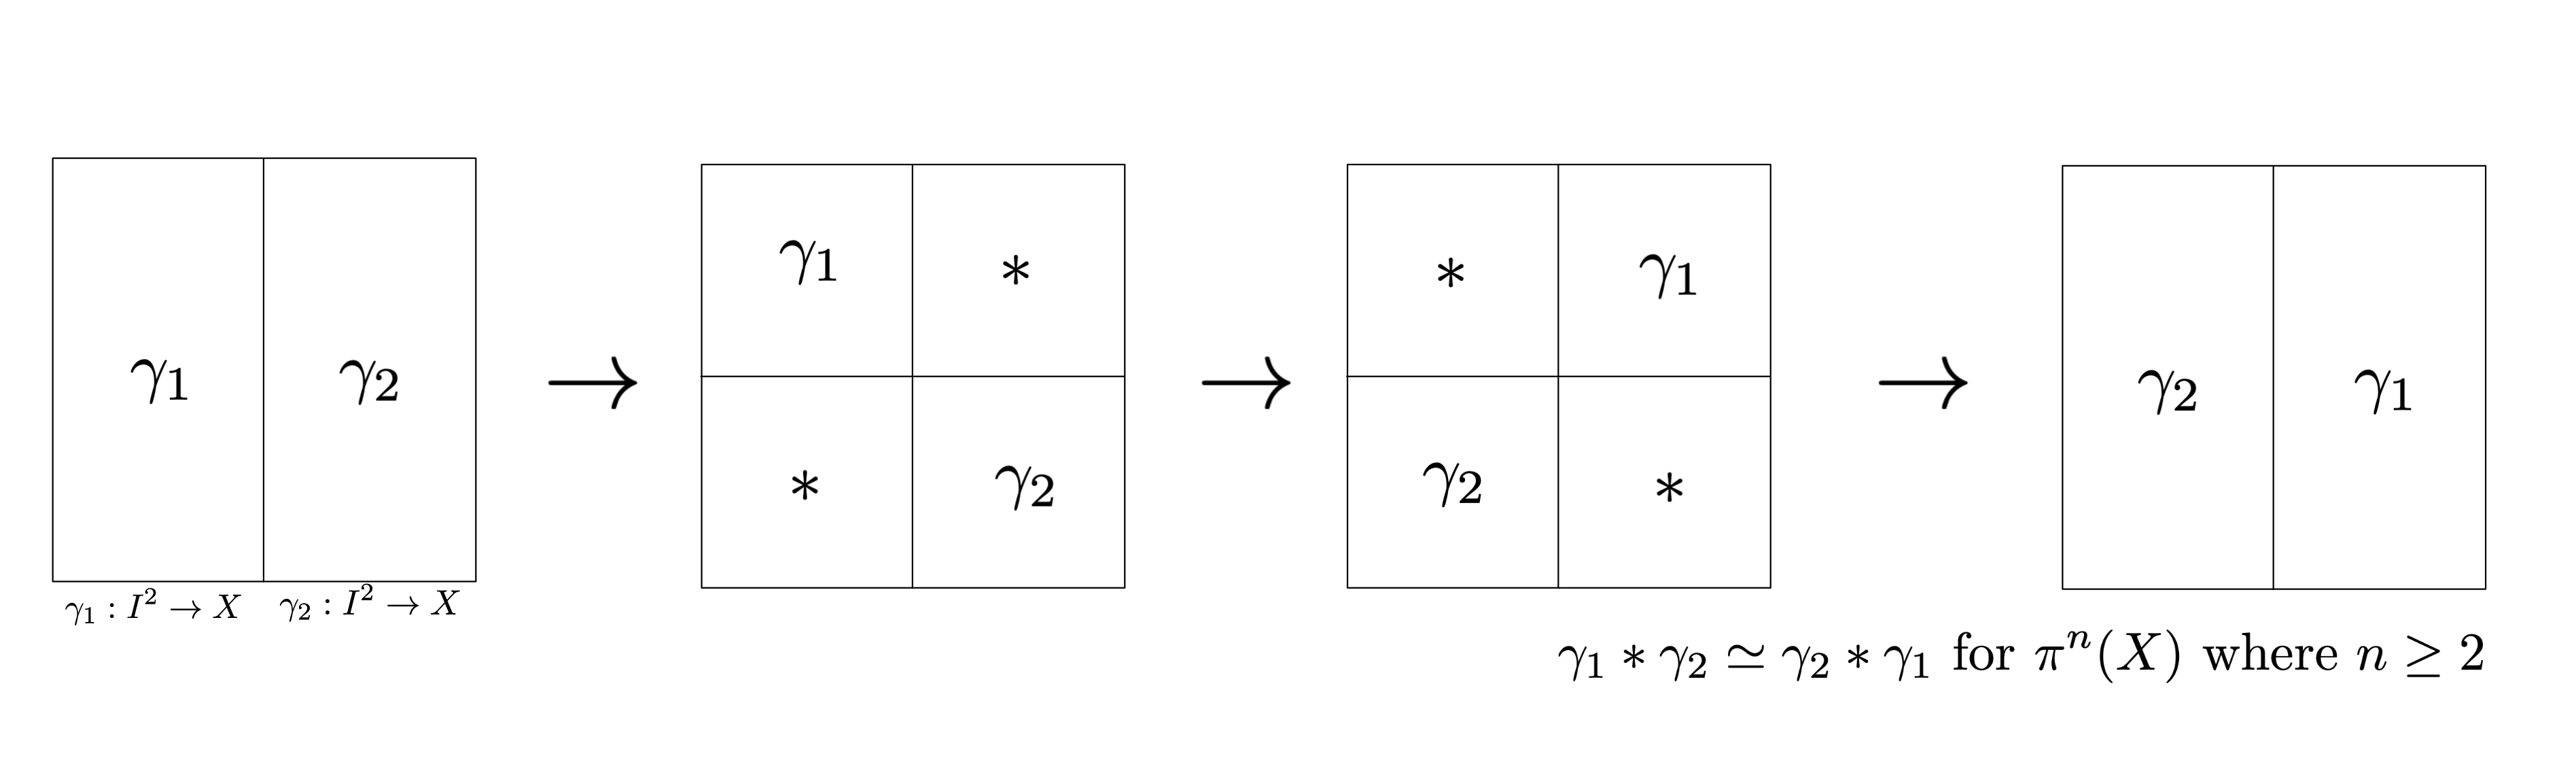
\includegraphics[width=\textwidth]{homotopygroupsabelian.png}
		\caption{A diagram of the homotopy of $I^2$ that proves that the homotopy groups of dimension 2 and above are Abelian}
	\end{figure}
	
	$[X,Y]$ is a set. $[\Sigma X, Y]$ is a group. $[\Sigma^2 X, Y]$ is a group, and it will continue to hold for $[\Sigma^n X, Y]$ for $n\geq 2$. Maps from $\Sigma^2 X\to Y$ is homeomorphic to maps from $X$ to $\Omega^2 Y$. Then $\Omega^2 X \to X$ is the same as the set of all maps form the square to $X$ which takes $\partial I^2$ to the basepoint. What's the homotopy? It's called the ``spin the wheel homotopy" for $\gamma_1\ast \gamma_2$ and $\gamma_2\ast \gamma_1$. Therefore homotopy classes of maps on the $I^2$ commute, so $[\Sigma^2 X, Y]$ is an Abelian group. 
	
	There are some unsettling facts here. Going from $0$ to $1$ loop took us from sets to groups, which is a vast jump (algae has srtarted walking on land) and then $1$ to $2$ goes to an Abelian group. Then after that we get nothing else. It increases wildly. This is the beginning of the theory of E-N Algebras
		Culinary indoctrination:
	B+H Diary, Veselka, Blue + Gold. B+H Dairy is a classic Dairy restaurant, the Blue + Gold is a bar, and Veselka is a 24 hour diner.
	
	Culinary questions: Food from city states or near city states. Any places that are good for Taiwanese or Singaporean food
	
	Long exact sequences of a cofiber sequence \begin{center}
		\begin{tikzcd}
		X\arrow[r] \arrow[d] &Y\arrow[d] \\ \ast \arrow[r] &Y/X
		\end{tikzcd}
	\end{center}
	Then $Y/X$ has a universal property with $Y\to Y/X$ in \begin{center}
		\begin{tikzcd}
		X\arrow[rr]\arrow[dr] && Y/X\arrow[dl]\\
		&Y
		\end{tikzcd}
	\end{center}
	
	Remember, we introduced $Cf$ as a homotopical proxy for $Y/X$:
	
	\begin{lemma}{1}
		If $x\rightarrowtail Y$ is a cofibration then $Y/X\simeq Cf$
	\end{lemma}
	\begin{proof}
		\begin{center}
			\begin{tikzcd}
			X\arrow[r] \arrow[d]&CX\arrow[d]\\
			Y\arrow[r] & Cf
			\end{tikzcd}
		\end{center}
		then $Y/X\cong Cf/CX\simeq Cf$
	\end{proof}
	
	But what is the universal property of $Cf$? \begin{center}
		\begin{tikzcd}
		X\arrow[r] & Y \arrow[r] & Cf
		\end{tikzcd}
	\end{center}
	This is null homotopic \begin{equation*}
	\begin{split}
	X\times I &\to Cf\\
	(x,t)&\mapsto (\ast,t)
	\end{split}
	\end{equation*}
	
	\begin{center}
		\begin{tikzcd}
		X\arrow[r] &Y \arrow[d] \\&Z
		\end{tikzcd}
		is null homotopic if and only if \
		\begin{tikzcd}
		X\arrow[r] \arrow[dr]& Y \arrow[r] \arrow[d]&Cf\arrow[dl,dashrightarrow]\\
		&	Z
		\end{tikzcd}
	\end{center}
	As an immediate consequence, given $Z$ and $X\to Y \to Cf$ has the exact sequence \[
	[Cf,Z]\to [Y,Z]\to [X,Z]
	\]
	is an exact sequence of sets. 
	
	We can write two sequences
	\begin{center}
		\begin{tikzcd}
		X\arrow[r] & Y \arrow[r] & Cf\arrow[r] & \Sigma X\arrow[r] & \Sigma Y \arrow[r] & C(\Sigma f)\arrow[r] & \Sigma^2X\arrow[r] &\Sigma^2Y\arrow[r] &\dots
		\end{tikzcd}\\
		\begin{tikzcd}
		X\arrow[r] & Y \arrow[r,"g_0"]\arrow[r] & Cf\arrow[r,"g_1"] & Cg_0\arrow[r]&Cg_1\arrow[r]&\dots
		\end{tikzcd}
	\end{center}
	Each term is the cofiber of the last, and so by this iteration it becomes clear that the second sequence gives rise to a long exact sequence when you apply $[-,Z]$. From the first sequence, we want to show that $[Cg_0,Z]\cong [\Sigma X,Z]$ and we want to show that there exists comparisons between the first sequence and the second which induce the same sequence on $[-,Z]$. Recall from last class that $[\Sigma X,Y]$ is a group and $[\Sigma^2 X,Y]$ is an Abelian group. 
	
	When considering iterated versions of this comparison, we can look at maps in $\Sigma^2 X$ and $\Sigma^2 f$ and these make a permutation
	\begin{center}
		\begin{tikzcd}
		X\arrow[r] \arrow[d,equal]& Y \arrow[r]\arrow[d,equal] & Cf\arrow[r]\arrow[d,equal] & \Sigma X\arrow[r] & \Sigma Y \arrow[r] & C(\Sigma f)\arrow[r]\arrow[d] & \Sigma^2X\arrow[r]\arrow[d,"\tau"] &\Sigma^2Y\arrow[r] \arrow[d]&C(\Sigma^2f)\arrow[r]&\dots\\
		
		X\arrow[r] & Y \arrow[r] & Cf\arrow[r] & \Sigma X\arrow[r] & \Sigma Y \arrow[r] & C(\Sigma f)\arrow[r] & \Sigma^2X\arrow[r] &\Sigma^2Y\arrow[r] &C(\Sigma^2f)\arrow[r]&\dots
		\end{tikzcd}\end{center}
	This sequence on homotopy gives rise to the LES of a pair $(A,X)$
	\begin{center}
		\begin{tikzcd}
		A\arrow[r,"f"]& X\arrow[r] &Cf\arrow[r]& \Sigma A\arrow[r] & \Sigma X\arrow[r]&\dots
		\end{tikzcd}
	\end{center}
	Then we can get that \[
	H_*(Cf)\cong H_*(Cf,CA)\cong H_*(X\times I, A\times I)\cong H_*(X,A)
	\]
	with the middle isomorphism by excision. 
	
	If $A\rightarrowtail X$ is a cofibration then $H_n(X,A)\cong H_n(X/A)\cong H_n(Cf)$. 
	
	As an aside, when you work in this context you get a lot of power that is homotopy invariant and we can use homotopy theory to solve our problems. On the other hand, it takes what you said and turns it into what the machinery thinks you wanted to say, but perhaps it doesn't say what you want it to say. From the perspective of this class homotopy is what we're studying, but often there's more important refined data that you want to keep. If you study manifolds or varities it is removing a lot of data to just studying it upto homotopy type. 
	
	We have been doing this in the context of the functor $[-,Z]$ since this is the relevant functor for the long exact sequence in homology. What about functors $[Z,-]$? Given a map $X\to Y$ can we form some kind of long exact sequence? We are now starting to follow up on our long intended 
	
	\begin{definition}
		If $X$ is a based space then \[
		\pi_n(X)=[S^n,X]
		\]
		Then we find that $\pi_0(X)$ is the path components, $\pi_1(X)$ is the fundamental group, and $\pi_n(X)$ are Abelian groups. 
	\end{definition}
	The Abelian group thing is very helpful, as there's a lot more known structure to Abelian groups. Homotopy groups are hard. Homology is pretty easy. We don't know what the homotopy groups of spheres are. 
	\begin{definition}
		$f:X\to Y$ is a weak equivalence if the induced map $\pi_nf:\pi_n(X)\to \pi_n(Y)$ is an isomorphism for all $n$. 
	\end{definition}
	We will eventually prove the following theorem
	\begin{theorem}
		If $f:X\to Y$ is a weak equivalence and $X,Y$ are CW complexes, then $f$ is a homotopy equivalence. 
	\end{theorem}
	As an aside, we can construct \textsf{Ho(Top)} by looking at CW complexes, category \textsf{D} and formally inverting to weak equivalences. This gives you a universal property through formal inversion. Functors out of CW complexes are functors out of \textsf{Ho(Top)}:\begin{center}
		\begin{tikzcd}
		\mathsf{Top}\arrow[rr]\arrow[dr]&&\mathsf{D}\arrow[dl]\\
		& \mathsf{Ho(Top)}
		\end{tikzcd}
	\end{center}
	The data of a weak equivalence involves the map $f$. It is not an abstract isomorphism of $f$. You have to have the map that induces the isomorphism of homotopy groups. There are examples of spaces with equal homotopy groups that are not homotopy equivalents. 
	
	As a question, is $\pi_*$ a homology theory, i.e. does it satisfy the Eilenberg-Steinrod axioms? Unfortunately the answer is no. 
	
	Suppose we relax the axiom that says that the value on a point is $\mathbb{Z}$ or $R$. (i.e. we generalize homology theories, other examples are topological k-theory or cobordism.) The value of any kind of theory like this is heavily constrained on spheres because of the suspension consequence of the axioms. That's just not true for homotopy groups. $\pi_1(S^1)=\mathbb{Z}$ and that's good but in general it is not the case that $\pi_n(S^k)$ is compatible with suspension. We know this for trivial reasons. Let's think about some things we know about homotopy groups. 
	
	\begin{lemma}{1}
		$\pi_k(S^n)=0$ for $k<n$. This is in some sense a result of differential topology. It will miss something and you can pull out a point and contract the resulting plane. 
	\end{lemma}
	We don't actually know $\pi_n(S^k)$ for most pairs $(n,k)$. We will spend some time talking about $\pi_3(S^2)$ which is not compatible with any kind of Eilenberg Steinrod type axioms.  
	
	Can we turn $\{\pi_*(-)]\}$ into a homotopy theory formally? If we had LES associated to a map $f:X\to Y$ in $[Z,-]$ then we might hope to get something like a LES in $\pi_*$. 
	
	$[\Sigma X,Z]$ and $[Z,\Omega^n X]$ has $\pi_0(\Omega^n X)\cong \pi_n(X)$. This is a reminder of the origin of the algebraic structure on $\pi_n(X)$. Now we will dualize the story of cofibrations, i.e. fibrations. 
	
	Cofibrations were answering the question ``how should we take the quotient?" Now we will think about the dual, where $X$ and $Y$ are based and we have $f^{-1}(\ast)\to X\to Y$ fiber. 
	\begin{center}
		\begin{tikzcd}
		F\arrow[r] \arrow[d] &X\arrow[d]\\
		\ast \arrow[r] &Y
		\end{tikzcd}
	\end{center}
	We get a fiber, which is the same question that we always ask. Is it the case that $F$ is homotopy invariant?  When is it?  The theory of fibrations will be when the fiber is a homotopy invariant. 
	\begin{center}
		\begin{tikzcd}
		\ast \arrow[r] \arrow[d,equal] & Y&\arrow[l]X\\
		\ast\arrow[r]& Y'\arrow[u,"cong"]&\arrow[l] X\arrow[u,"\cong"]
		\end{tikzcd}
	\end{center}

\end{document}